\documentclass[twoside]{book}

% Packages required by doxygen
\usepackage{fixltx2e}
\usepackage{calc}
\usepackage{doxygen}
\usepackage[export]{adjustbox} % also loads graphicx
\usepackage{graphicx}
\usepackage[utf8]{inputenc}
\usepackage{makeidx}
\usepackage{multicol}
\usepackage{multirow}
\PassOptionsToPackage{warn}{textcomp}
\usepackage{textcomp}
\usepackage[nointegrals]{wasysym}
\usepackage[table]{xcolor}

% Font selection
\usepackage[T1]{fontenc}
\usepackage[scaled=.90]{helvet}
\usepackage{courier}
\usepackage{amssymb}
\usepackage{sectsty}
\renewcommand{\familydefault}{\sfdefault}
\allsectionsfont{%
  \fontseries{bc}\selectfont%
  \color{darkgray}%
}
\renewcommand{\DoxyLabelFont}{%
  \fontseries{bc}\selectfont%
  \color{darkgray}%
}
\newcommand{\+}{\discretionary{\mbox{\scriptsize$\hookleftarrow$}}{}{}}

% Page & text layout
\usepackage{geometry}
\geometry{%
  a4paper,%
  top=2.5cm,%
  bottom=2.5cm,%
  left=2.5cm,%
  right=2.5cm%
}
\tolerance=750
\hfuzz=15pt
\hbadness=750
\setlength{\emergencystretch}{15pt}
\setlength{\parindent}{0cm}
\setlength{\parskip}{3ex plus 2ex minus 2ex}
\makeatletter
\renewcommand{\paragraph}{%
  \@startsection{paragraph}{4}{0ex}{-1.0ex}{1.0ex}{%
    \normalfont\normalsize\bfseries\SS@parafont%
  }%
}
\renewcommand{\subparagraph}{%
  \@startsection{subparagraph}{5}{0ex}{-1.0ex}{1.0ex}{%
    \normalfont\normalsize\bfseries\SS@subparafont%
  }%
}
\makeatother

% Headers & footers
\usepackage{fancyhdr}
\pagestyle{fancyplain}
\fancyhead[LE]{\fancyplain{}{\bfseries\thepage}}
\fancyhead[CE]{\fancyplain{}{}}
\fancyhead[RE]{\fancyplain{}{\bfseries\leftmark}}
\fancyhead[LO]{\fancyplain{}{\bfseries\rightmark}}
\fancyhead[CO]{\fancyplain{}{}}
\fancyhead[RO]{\fancyplain{}{\bfseries\thepage}}
\fancyfoot[LE]{\fancyplain{}{}}
\fancyfoot[CE]{\fancyplain{}{}}
\fancyfoot[RE]{\fancyplain{}{\bfseries\scriptsize Generated by Doxygen }}
\fancyfoot[LO]{\fancyplain{}{\bfseries\scriptsize Generated by Doxygen }}
\fancyfoot[CO]{\fancyplain{}{}}
\fancyfoot[RO]{\fancyplain{}{}}
\renewcommand{\footrulewidth}{0.4pt}
\renewcommand{\chaptermark}[1]{%
  \markboth{#1}{}%
}
\renewcommand{\sectionmark}[1]{%
  \markright{\thesection\ #1}%
}

% Indices & bibliography
\usepackage{natbib}
\usepackage[titles]{tocloft}
\setcounter{tocdepth}{3}
\setcounter{secnumdepth}{5}
\makeindex

% Hyperlinks (required, but should be loaded last)
\usepackage{ifpdf}
\ifpdf
  \usepackage[pdftex,pagebackref=true]{hyperref}
\else
  \usepackage[ps2pdf,pagebackref=true]{hyperref}
\fi
\hypersetup{%
  colorlinks=true,%
  linkcolor=blue,%
  citecolor=blue,%
  unicode%
}

% Custom commands
\newcommand{\clearemptydoublepage}{%
  \newpage{\pagestyle{empty}\cleardoublepage}%
}

\usepackage{caption}
\captionsetup{labelsep=space,justification=centering,font={bf},singlelinecheck=off,skip=4pt,position=top}

%===== C O N T E N T S =====

\begin{document}

% Titlepage & ToC
\hypersetup{pageanchor=false,
             bookmarksnumbered=true,
             pdfencoding=unicode
            }
\pagenumbering{roman}
\begin{titlepage}
\vspace*{7cm}
\begin{center}%
{\Large My Project }\\
\vspace*{1cm}
{\large Generated by Doxygen 1.8.11}\\
\end{center}
\end{titlepage}
\clearemptydoublepage
\tableofcontents
\clearemptydoublepage
\pagenumbering{arabic}
\hypersetup{pageanchor=true}

%--- Begin generated contents ---
\chapter{Class Index}
\section{Class List}
Here are the classes, structs, unions and interfaces with brief descriptions\+:\begin{DoxyCompactList}
\item\contentsline{section}{\hyperlink{structadd__entry}{add\+\_\+entry} }{\pageref{structadd__entry}}{}
\item\contentsline{section}{\hyperlink{structbuckets}{buckets} }{\pageref{structbuckets}}{}
\item\contentsline{section}{\hyperlink{structentry}{entry} }{\pageref{structentry}}{}
\item\contentsline{section}{\hyperlink{structentry__args}{entry\+\_\+args} }{\pageref{structentry__args}}{}
\item\contentsline{section}{\hyperlink{structhashmap__args}{hashmap\+\_\+args} }{\pageref{structhashmap__args}}{}
\item\contentsline{section}{\hyperlink{structhashmap__atomic}{hashmap\+\_\+atomic} }{\pageref{structhashmap__atomic}}{}
\item\contentsline{section}{\hyperlink{structhashmap__rp}{hashmap\+\_\+rp} }{\pageref{structhashmap__rp}}{}
\item\contentsline{section}{\hyperlink{structhashmap__tx}{hashmap\+\_\+tx} }{\pageref{structhashmap__tx}}{}
\end{DoxyCompactList}

\chapter{File Index}
\section{File List}
Here is a list of all documented files with brief descriptions\+:\begin{DoxyCompactList}
\item\contentsline{section}{\hyperlink{hashmap_8h}{hashmap.\+h} \\*Hashmap implementation in persistent memory }{\pageref{hashmap_8h}}{}
\item\contentsline{section}{\hyperlink{hashmap__atomic_8h}{hashmap\+\_\+atomic.\+h} \\*Implementation of atomic hashmap, where inserts are coordinated to be one after the other }{\pageref{hashmap__atomic_8h}}{}
\item\contentsline{section}{{\bfseries hashmap\+\_\+internal.\+h} }{\pageref{hashmap__internal_8h}}{}
\item\contentsline{section}{{\bfseries hashmap\+\_\+rp.\+h} }{\pageref{hashmap__rp_8h}}{}
\item\contentsline{section}{{\bfseries hashmap\+\_\+tx.\+h} }{\pageref{hashmap__tx_8h}}{}
\end{DoxyCompactList}

\chapter{Class Documentation}
\hypertarget{structadd__entry}{}\section{add\+\_\+entry Struct Reference}
\label{structadd__entry}\index{add\+\_\+entry@{add\+\_\+entry}}


Collaboration diagram for add\+\_\+entry\+:
% FIG 0
\subsection*{Public Attributes}
\begin{DoxyCompactItemize}
\item 
\mbox{\Hypertarget{structadd__entry_ada303ac47bbd298d31a08ff5fb0c8d48}\label{structadd__entry_ada303ac47bbd298d31a08ff5fb0c8d48}} 
struct \hyperlink{structentry}{entry} {\bfseries data}
\item 
\mbox{\Hypertarget{structadd__entry_aff20888396f928a47207ec2fe432efe9}\label{structadd__entry_aff20888396f928a47207ec2fe432efe9}} 
size\+\_\+t {\bfseries pos}
\item 
\mbox{\Hypertarget{structadd__entry_a02a8967aa6cd3e8bbbaa6c35571379a2}\label{structadd__entry_a02a8967aa6cd3e8bbbaa6c35571379a2}} 
struct pobj\+\_\+action $\ast$ {\bfseries actv}
\item 
\mbox{\Hypertarget{structadd__entry_a288eb722a38cd8a357d0600475defe70}\label{structadd__entry_a288eb722a38cd8a357d0600475defe70}} 
size\+\_\+t {\bfseries actv\+\_\+cnt}
\end{DoxyCompactItemize}


The documentation for this struct was generated from the following file\+:\begin{DoxyCompactItemize}
\item 
hashmap/hashmap\+\_\+rp.\+c\end{DoxyCompactItemize}

\hypertarget{structbuckets}{}\section{buckets Struct Reference}
\label{structbuckets}\index{buckets@{buckets}}
\subsection*{Public Attributes}
\begin{DoxyCompactItemize}
\item 
\mbox{\Hypertarget{structbuckets_ab4b1efc42ff06fef401feb5297469441}\label{structbuckets_ab4b1efc42ff06fef401feb5297469441}} 
size\+\_\+t {\bfseries nbuckets}
\item 
\mbox{\Hypertarget{structbuckets_a563609796b380211a16c9f0eb07c4ff6}\label{structbuckets_a563609796b380211a16c9f0eb07c4ff6}} 
struct entries\+\_\+head {\bfseries bucket} \mbox{[}$\,$\mbox{]}
\end{DoxyCompactItemize}


The documentation for this struct was generated from the following files\+:\begin{DoxyCompactItemize}
\item 
hashmap/hashmap\+\_\+atomic.\+c\item 
hashmap/hashmap\+\_\+tx.\+c\end{DoxyCompactItemize}

\hypertarget{structentry}{}\section{entry Struct Reference}
\label{structentry}\index{entry@{entry}}


Collaboration diagram for entry\+:
% FIG 0
\subsection*{Public Attributes}
\begin{DoxyCompactItemize}
\item 
\mbox{\Hypertarget{structentry_a9baabf5b8c35d0a925340cd73e23ae8d}\label{structentry_a9baabf5b8c35d0a925340cd73e23ae8d}} 
uint64\+\_\+t {\bfseries key}
\item 
\mbox{\Hypertarget{structentry_abc6a75d6690199042034e9300aebd4c1}\label{structentry_abc6a75d6690199042034e9300aebd4c1}} 
\hyperlink{structpmemoid}{P\+M\+E\+Moid} {\bfseries value}
\item 
\mbox{\Hypertarget{structentry_a97cd1dbcdcea14e94f70a86a391b662b}\label{structentry_a97cd1dbcdcea14e94f70a86a391b662b}} 
uint64\+\_\+t {\bfseries hash}
\item 
\mbox{\Hypertarget{structentry_a8ac9b199255dffa2da0510ee7f85c4e4}\label{structentry_a8ac9b199255dffa2da0510ee7f85c4e4}} 
size\+\_\+t {\bfseries len}
\item 
\mbox{\Hypertarget{structentry_aaf5d81a7428014e8bb4711f33ff134eb}\label{structentry_aaf5d81a7428014e8bb4711f33ff134eb}} 
char {\bfseries data} \mbox{[}$\,$\mbox{]}
\end{DoxyCompactItemize}


The documentation for this struct was generated from the following files\+:\begin{DoxyCompactItemize}
\item 
hashmap/hashmap\+\_\+atomic.\+c\item 
hashmap/hashmap\+\_\+rp.\+c\item 
hashmap/hashmap\+\_\+tx.\+c\item 
queue/queue.\+c\end{DoxyCompactItemize}

\hypertarget{structentry__args}{}\section{entry\+\_\+args Struct Reference}
\label{structentry__args}\index{entry\+\_\+args@{entry\+\_\+args}}
\subsection*{Public Attributes}
\begin{DoxyCompactItemize}
\item 
uint64\+\_\+t {\bfseries key}\hypertarget{structentry__args_aba46158e3af0f0f4701ea742f7e05697}{}\label{structentry__args_aba46158e3af0f0f4701ea742f7e05697}

\item 
P\+M\+E\+Moid {\bfseries value}\hypertarget{structentry__args_a8a910e88fcd1bb7d94aa52080d6abb08}{}\label{structentry__args_a8a910e88fcd1bb7d94aa52080d6abb08}

\end{DoxyCompactItemize}


The documentation for this struct was generated from the following file\+:\begin{DoxyCompactItemize}
\item 
hashmap\+\_\+atomic.\+c\end{DoxyCompactItemize}

\hypertarget{structhashmap__args}{}\section{hashmap\+\_\+args Struct Reference}
\label{structhashmap__args}\index{hashmap\+\_\+args@{hashmap\+\_\+args}}
\subsection*{Public Attributes}
\begin{DoxyCompactItemize}
\item 
uint32\+\_\+t {\bfseries seed}\hypertarget{structhashmap__args_ae512628a8f83e3c1fca257201607b529}{}\label{structhashmap__args_ae512628a8f83e3c1fca257201607b529}

\end{DoxyCompactItemize}


The documentation for this struct was generated from the following file\+:\begin{DoxyCompactItemize}
\item 
\hyperlink{hashmap_8h}{hashmap.\+h}\end{DoxyCompactItemize}

\hypertarget{structhashmap__atomic}{}\section{hashmap\+\_\+atomic Struct Reference}
\label{structhashmap__atomic}\index{hashmap\+\_\+atomic@{hashmap\+\_\+atomic}}
\subsection*{Public Attributes}
\begin{DoxyCompactItemize}
\item 
\mbox{\Hypertarget{structhashmap__atomic_a83e3b765935189ca4a6bf0c0e33c8d09}\label{structhashmap__atomic_a83e3b765935189ca4a6bf0c0e33c8d09}} 
uint32\+\_\+t {\bfseries seed}
\item 
\mbox{\Hypertarget{structhashmap__atomic_a95d74f846934cb275183a28df0ff14a8}\label{structhashmap__atomic_a95d74f846934cb275183a28df0ff14a8}} 
uint32\+\_\+t {\bfseries hash\+\_\+fun\+\_\+a}
\item 
\mbox{\Hypertarget{structhashmap__atomic_aa2476a3fa7d4d13c4b4d83d80ee1bb4c}\label{structhashmap__atomic_aa2476a3fa7d4d13c4b4d83d80ee1bb4c}} 
uint32\+\_\+t {\bfseries hash\+\_\+fun\+\_\+b}
\item 
\mbox{\Hypertarget{structhashmap__atomic_ae9459faea29e49b192e2c2d8e59d235d}\label{structhashmap__atomic_ae9459faea29e49b192e2c2d8e59d235d}} 
uint64\+\_\+t {\bfseries hash\+\_\+fun\+\_\+p}
\item 
\mbox{\Hypertarget{structhashmap__atomic_adb45831ae8cc7d5335b048ccc0ba2009}\label{structhashmap__atomic_adb45831ae8cc7d5335b048ccc0ba2009}} 
uint64\+\_\+t {\bfseries count}
\item 
\mbox{\Hypertarget{structhashmap__atomic_a4e9b4e9443278085568203af85278e6f}\label{structhashmap__atomic_a4e9b4e9443278085568203af85278e6f}} 
uint32\+\_\+t {\bfseries count\+\_\+dirty}
\end{DoxyCompactItemize}


The documentation for this struct was generated from the following file\+:\begin{DoxyCompactItemize}
\item 
hashmap/hashmap\+\_\+atomic.\+c\end{DoxyCompactItemize}

\hypertarget{structhashmap__rp}{}\section{hashmap\+\_\+rp Struct Reference}
\label{structhashmap__rp}\index{hashmap\+\_\+rp@{hashmap\+\_\+rp}}
\subsection*{Public Attributes}
\begin{DoxyCompactItemize}
\item 
uint64\+\_\+t {\bfseries count}\hypertarget{structhashmap__rp_ab6c1dfb752de6101545bb92dcccc419a}{}\label{structhashmap__rp_ab6c1dfb752de6101545bb92dcccc419a}

\item 
uint64\+\_\+t {\bfseries capacity}\hypertarget{structhashmap__rp_a964fc2490d30dc7a73328999f7759076}{}\label{structhashmap__rp_a964fc2490d30dc7a73328999f7759076}

\item 
uint64\+\_\+t {\bfseries resize\+\_\+threshold}\hypertarget{structhashmap__rp_afcf78d28515e6c63cddd440e5b02c79c}{}\label{structhashmap__rp_afcf78d28515e6c63cddd440e5b02c79c}

\end{DoxyCompactItemize}


The documentation for this struct was generated from the following file\+:\begin{DoxyCompactItemize}
\item 
hashmap\+\_\+rp.\+c\end{DoxyCompactItemize}

\hypertarget{structhashmap__tx}{}\section{hashmap\+\_\+tx Struct Reference}
\label{structhashmap__tx}\index{hashmap\+\_\+tx@{hashmap\+\_\+tx}}
\subsection*{Public Attributes}
\begin{DoxyCompactItemize}
\item 
uint32\+\_\+t {\bfseries seed}\hypertarget{structhashmap__tx_a3a3693aa60920c724a0f4511b18a6fd2}{}\label{structhashmap__tx_a3a3693aa60920c724a0f4511b18a6fd2}

\item 
uint32\+\_\+t {\bfseries hash\+\_\+fun\+\_\+a}\hypertarget{structhashmap__tx_aff7708436836d0ae87500fa876dfcecf}{}\label{structhashmap__tx_aff7708436836d0ae87500fa876dfcecf}

\item 
uint32\+\_\+t {\bfseries hash\+\_\+fun\+\_\+b}\hypertarget{structhashmap__tx_a9f6c8ffb7a4f3472edb7afeb99e45074}{}\label{structhashmap__tx_a9f6c8ffb7a4f3472edb7afeb99e45074}

\item 
uint64\+\_\+t {\bfseries hash\+\_\+fun\+\_\+p}\hypertarget{structhashmap__tx_adc5b9769a040542bda4f25e3098f2837}{}\label{structhashmap__tx_adc5b9769a040542bda4f25e3098f2837}

\item 
uint64\+\_\+t {\bfseries count}\hypertarget{structhashmap__tx_a70fbb5e277e0e52c199c1024cfbd08c1}{}\label{structhashmap__tx_a70fbb5e277e0e52c199c1024cfbd08c1}

\end{DoxyCompactItemize}


The documentation for this struct was generated from the following file\+:\begin{DoxyCompactItemize}
\item 
hashmap\+\_\+tx.\+c\end{DoxyCompactItemize}

\chapter{File Documentation}
\hypertarget{hashmap_8h}{}\section{hashmap.\+h File Reference}
\label{hashmap_8h}\index{hashmap.\+h@{hashmap.\+h}}


Hashmap implementation in persistent memory.  


{\ttfamily \#include $<$stddef.\+h$>$}\\*
{\ttfamily \#include $<$stdint.\+h$>$}\\*
Include dependency graph for hashmap.\+h\+:\nopagebreak
\begin{figure}[H]
\begin{center}
\leavevmode
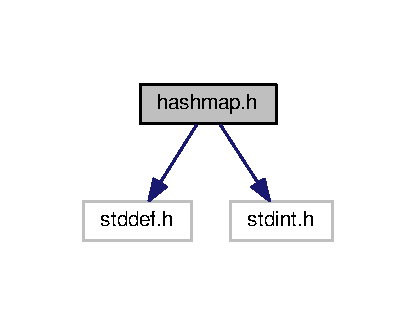
\includegraphics[width=200pt]{hashmap_8h__incl}
\end{center}
\end{figure}
This graph shows which files directly or indirectly include this file\+:
\nopagebreak
\begin{figure}[H]
\begin{center}
\leavevmode
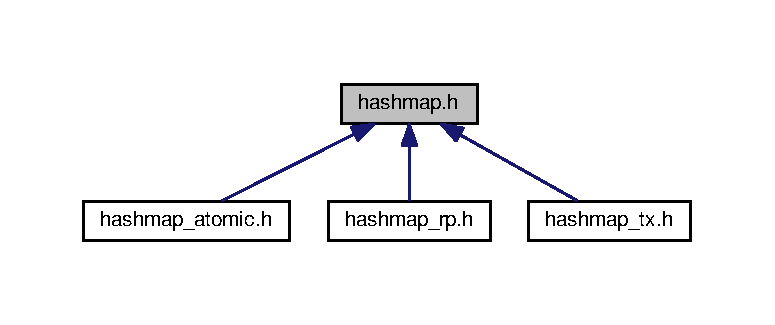
\includegraphics[width=350pt]{hashmap_8h__dep__incl}
\end{center}
\end{figure}
\subsection*{Classes}
\begin{DoxyCompactItemize}
\item 
struct \hyperlink{structhashmap__args}{hashmap\+\_\+args}
\end{DoxyCompactItemize}
\subsection*{Enumerations}
\begin{DoxyCompactItemize}
\item 
enum {\bfseries hashmap\+\_\+cmd} \{ {\bfseries H\+A\+S\+H\+M\+A\+P\+\_\+\+C\+M\+D\+\_\+\+R\+E\+B\+U\+I\+LD}, 
{\bfseries H\+A\+S\+H\+M\+A\+P\+\_\+\+C\+M\+D\+\_\+\+D\+E\+B\+UG}
 \}\hypertarget{hashmap_8h_a06616991d22cc27ebd6f17d026241386}{}\label{hashmap_8h_a06616991d22cc27ebd6f17d026241386}

\end{DoxyCompactItemize}


\subsection{Detailed Description}
Hashmap implementation in persistent memory. 

Details. 
\hypertarget{hashmap__atomic_8h}{}\section{hashmap/hashmap\+\_\+atomic.h File Reference}
\label{hashmap__atomic_8h}\index{hashmap/hashmap\+\_\+atomic.\+h@{hashmap/hashmap\+\_\+atomic.\+h}}


Implementation of atomic hashmap, where inserts are coordinated to be one after the other.  


{\ttfamily \#include $<$stddef.\+h$>$}\newline
{\ttfamily \#include $<$stdint.\+h$>$}\newline
{\ttfamily \#include $<$hashmap.\+h$>$}\newline
{\ttfamily \#include $<$libpmemobj.\+h$>$}\newline
Include dependency graph for hashmap\+\_\+atomic.\+h\+:
% FIG 0
\subsection*{Macros}
\begin{DoxyCompactItemize}
\item 
\mbox{\Hypertarget{hashmap__atomic_8h_ac7a2806ad6610fce7f1a06b8777c773f}\label{hashmap__atomic_8h_ac7a2806ad6610fce7f1a06b8777c773f}} 
\#define {\bfseries H\+A\+S\+H\+M\+A\+P\+\_\+\+A\+T\+O\+M\+I\+C\+\_\+\+T\+Y\+P\+E\+\_\+\+O\+F\+F\+S\+ET}~1000
\end{DoxyCompactItemize}
\subsection*{Functions}
\begin{DoxyCompactItemize}
\item 
\mbox{\Hypertarget{hashmap__atomic_8h_a10298cea42cfb536c27f9c6a4abeecc1}\label{hashmap__atomic_8h_a10298cea42cfb536c27f9c6a4abeecc1}} 
{\bfseries T\+O\+I\+D\+\_\+\+D\+E\+C\+L\+A\+RE} (struct \hyperlink{structhashmap__atomic}{hashmap\+\_\+atomic}, H\+A\+S\+H\+M\+A\+P\+\_\+\+A\+T\+O\+M\+I\+C\+\_\+\+T\+Y\+P\+E\+\_\+\+O\+F\+F\+S\+ET+0)
\item 
\mbox{\Hypertarget{hashmap__atomic_8h_a598708b91dce5756734872ba7591f275}\label{hashmap__atomic_8h_a598708b91dce5756734872ba7591f275}} 
int {\bfseries hm\+\_\+atomic\+\_\+check} (P\+M\+E\+Mobjpool $\ast$pop, T\+O\+ID(struct \hyperlink{structhashmap__atomic}{hashmap\+\_\+atomic}) hashmap)
\item 
\mbox{\Hypertarget{hashmap__atomic_8h_acbb4c401a679ca192b8758cde9befce8}\label{hashmap__atomic_8h_acbb4c401a679ca192b8758cde9befce8}} 
int {\bfseries hm\+\_\+atomic\+\_\+create} (P\+M\+E\+Mobjpool $\ast$pop, T\+O\+ID(struct \hyperlink{structhashmap__atomic}{hashmap\+\_\+atomic}) $\ast$map, void $\ast$arg)
\item 
\mbox{\Hypertarget{hashmap__atomic_8h_a04f0c019c9846769951407ba5a03fb16}\label{hashmap__atomic_8h_a04f0c019c9846769951407ba5a03fb16}} 
int {\bfseries hm\+\_\+atomic\+\_\+init} (P\+M\+E\+Mobjpool $\ast$pop, T\+O\+ID(struct \hyperlink{structhashmap__atomic}{hashmap\+\_\+atomic}) hashmap)
\item 
\mbox{\Hypertarget{hashmap__atomic_8h_af9e2aa6113e1ce3b5dbaac973ebda554}\label{hashmap__atomic_8h_af9e2aa6113e1ce3b5dbaac973ebda554}} 
int {\bfseries hm\+\_\+atomic\+\_\+insert} (P\+M\+E\+Mobjpool $\ast$pop, T\+O\+ID(struct \hyperlink{structhashmap__atomic}{hashmap\+\_\+atomic}) hashmap, uint64\+\_\+t key, \hyperlink{structpmemoid}{P\+M\+E\+Moid} value)
\item 
\mbox{\Hypertarget{hashmap__atomic_8h_a271644b8a80804a39314ce6cf7582b33}\label{hashmap__atomic_8h_a271644b8a80804a39314ce6cf7582b33}} 
\hyperlink{structpmemoid}{P\+M\+E\+Moid} {\bfseries hm\+\_\+atomic\+\_\+remove} (P\+M\+E\+Mobjpool $\ast$pop, T\+O\+ID(struct \hyperlink{structhashmap__atomic}{hashmap\+\_\+atomic}) hashmap, uint64\+\_\+t key)
\item 
\mbox{\Hypertarget{hashmap__atomic_8h_ad203219cd5cd5a4d69661004b53f193f}\label{hashmap__atomic_8h_ad203219cd5cd5a4d69661004b53f193f}} 
\hyperlink{structpmemoid}{P\+M\+E\+Moid} {\bfseries hm\+\_\+atomic\+\_\+get} (P\+M\+E\+Mobjpool $\ast$pop, T\+O\+ID(struct \hyperlink{structhashmap__atomic}{hashmap\+\_\+atomic}) hashmap, uint64\+\_\+t key)
\item 
\mbox{\Hypertarget{hashmap__atomic_8h_aaf062e36e2b6e22bc832847d5ee67dd1}\label{hashmap__atomic_8h_aaf062e36e2b6e22bc832847d5ee67dd1}} 
int {\bfseries hm\+\_\+atomic\+\_\+lookup} (P\+M\+E\+Mobjpool $\ast$pop, T\+O\+ID(struct \hyperlink{structhashmap__atomic}{hashmap\+\_\+atomic}) hashmap, uint64\+\_\+t key)
\item 
\mbox{\Hypertarget{hashmap__atomic_8h_af1a055b49bce902e78ef3774e6ea5918}\label{hashmap__atomic_8h_af1a055b49bce902e78ef3774e6ea5918}} 
int {\bfseries hm\+\_\+atomic\+\_\+foreach} (P\+M\+E\+Mobjpool $\ast$pop, T\+O\+ID(struct \hyperlink{structhashmap__atomic}{hashmap\+\_\+atomic}) hashmap, int($\ast$cb)(uint64\+\_\+t key, \hyperlink{structpmemoid}{P\+M\+E\+Moid} value, void $\ast$arg), void $\ast$arg)
\item 
\mbox{\Hypertarget{hashmap__atomic_8h_a6cb2f755fcf3b9b7c0361754ce6444ce}\label{hashmap__atomic_8h_a6cb2f755fcf3b9b7c0361754ce6444ce}} 
size\+\_\+t {\bfseries hm\+\_\+atomic\+\_\+count} (P\+M\+E\+Mobjpool $\ast$pop, T\+O\+ID(struct \hyperlink{structhashmap__atomic}{hashmap\+\_\+atomic}) hashmap)
\item 
\mbox{\Hypertarget{hashmap__atomic_8h_a1b44897be6a25691a516e1af2d2a2e26}\label{hashmap__atomic_8h_a1b44897be6a25691a516e1af2d2a2e26}} 
int {\bfseries hm\+\_\+atomic\+\_\+cmd} (P\+M\+E\+Mobjpool $\ast$pop, T\+O\+ID(struct \hyperlink{structhashmap__atomic}{hashmap\+\_\+atomic}) hashmap, unsigned cmd, uint64\+\_\+t arg)
\end{DoxyCompactItemize}


\subsection{Detailed Description}
Implementation of atomic hashmap, where inserts are coordinated to be one after the other. 

Details. 
%--- End generated contents ---

% Index
\backmatter
\newpage
\phantomsection
\clearemptydoublepage
\addcontentsline{toc}{chapter}{Index}
\printindex

\end{document}
